\section{The Digital Receiver}
\subsection{RF Chain}
\label{sec:digitalRX}

\begin{figure}[ht]
 \centering
 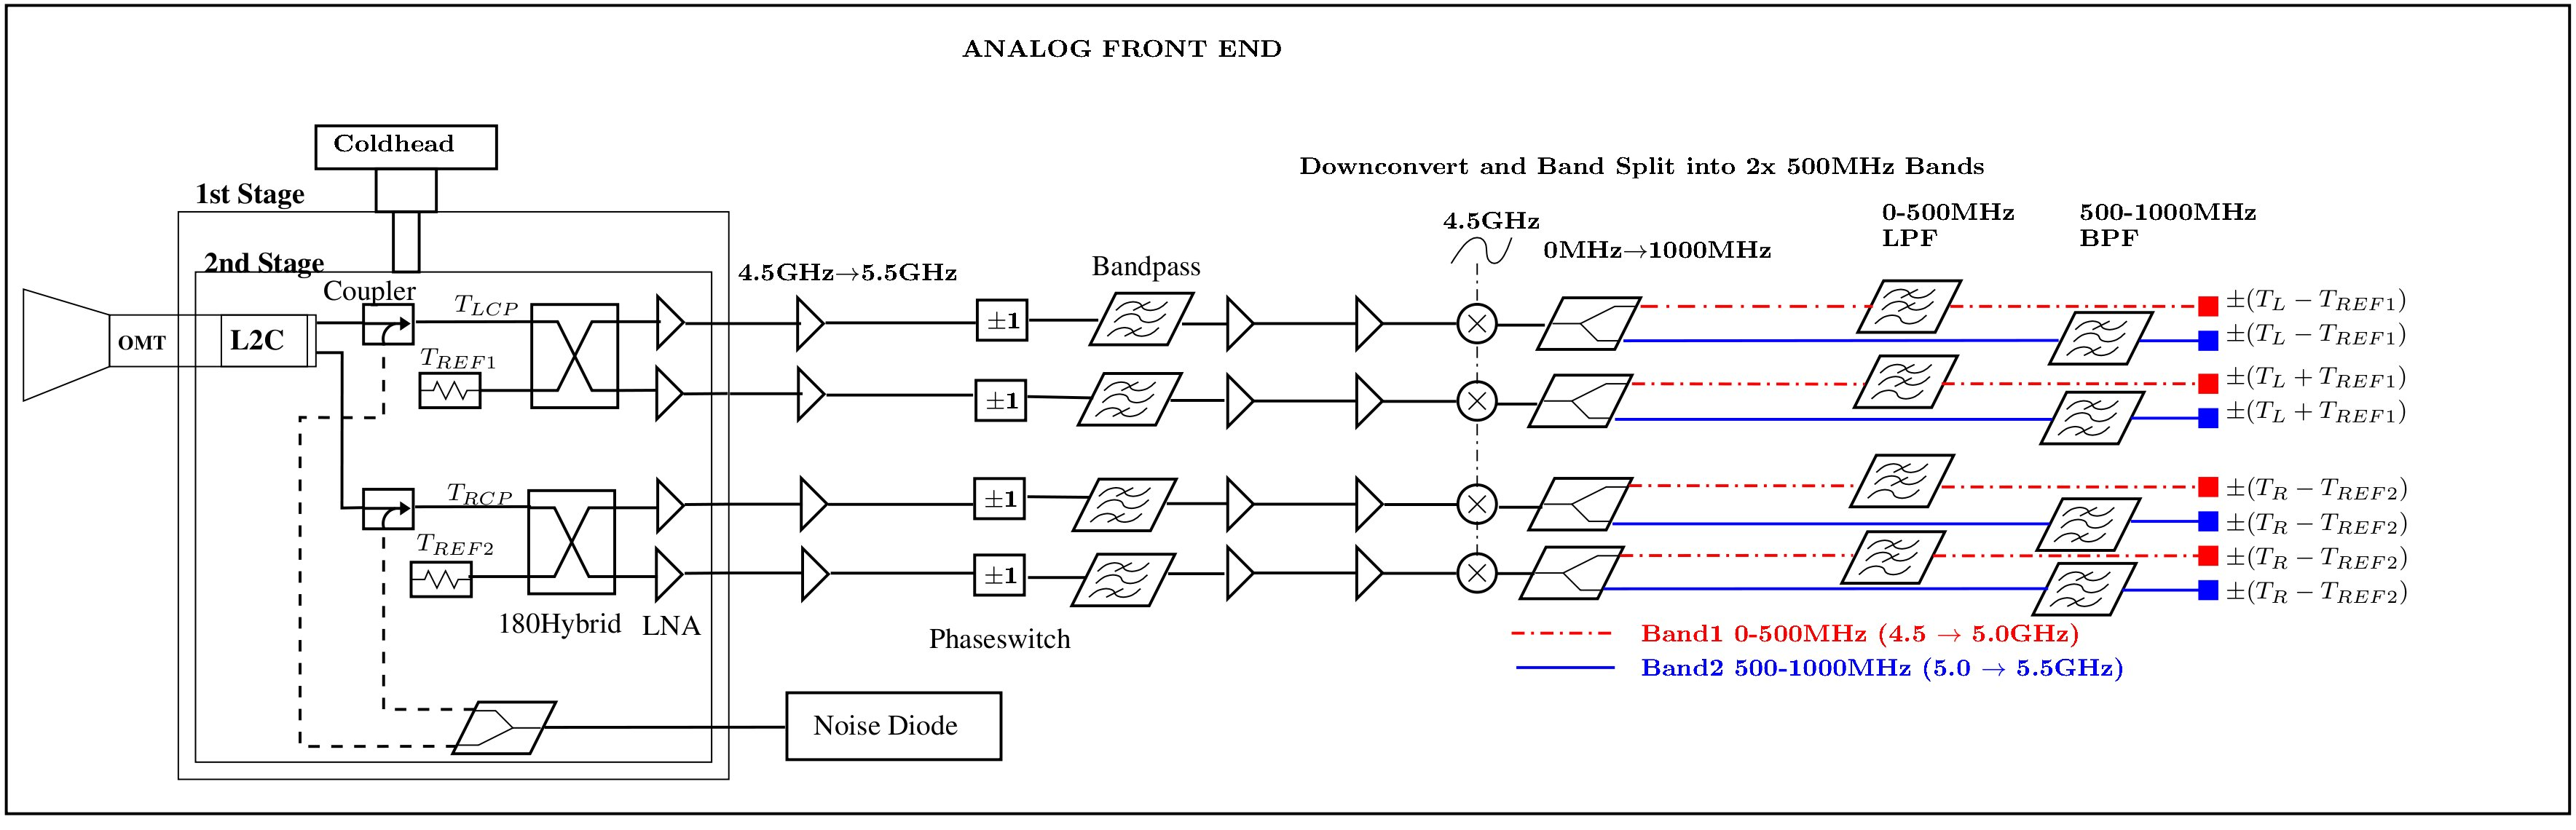
\includegraphics[width=\textwidth,height=0.4\textheight]{images/receiver_schematics/rfNew.jpg} % analog.png: 1920x1200 pixel, 72dpi, 67.73x42.33 cm, bb=
 \caption{Diagram of the analog front end of the digital receiver. There are significantly fewer analog components than the Northern Hemisphere polarimeter (see \appen{sec:pseudoCorrelation}, \fign{fig:analog_receiver}). The diagram shows the down-conversion of the 1~GHz band (into two 500~MHz bands) followed by the ADC capture. The digital processing is shown on \fign{fig:digital_receiver_mine}  }
 \label{fig:digital_receiver}
\end{figure}

\begin{figure}[ht]
 \centering
 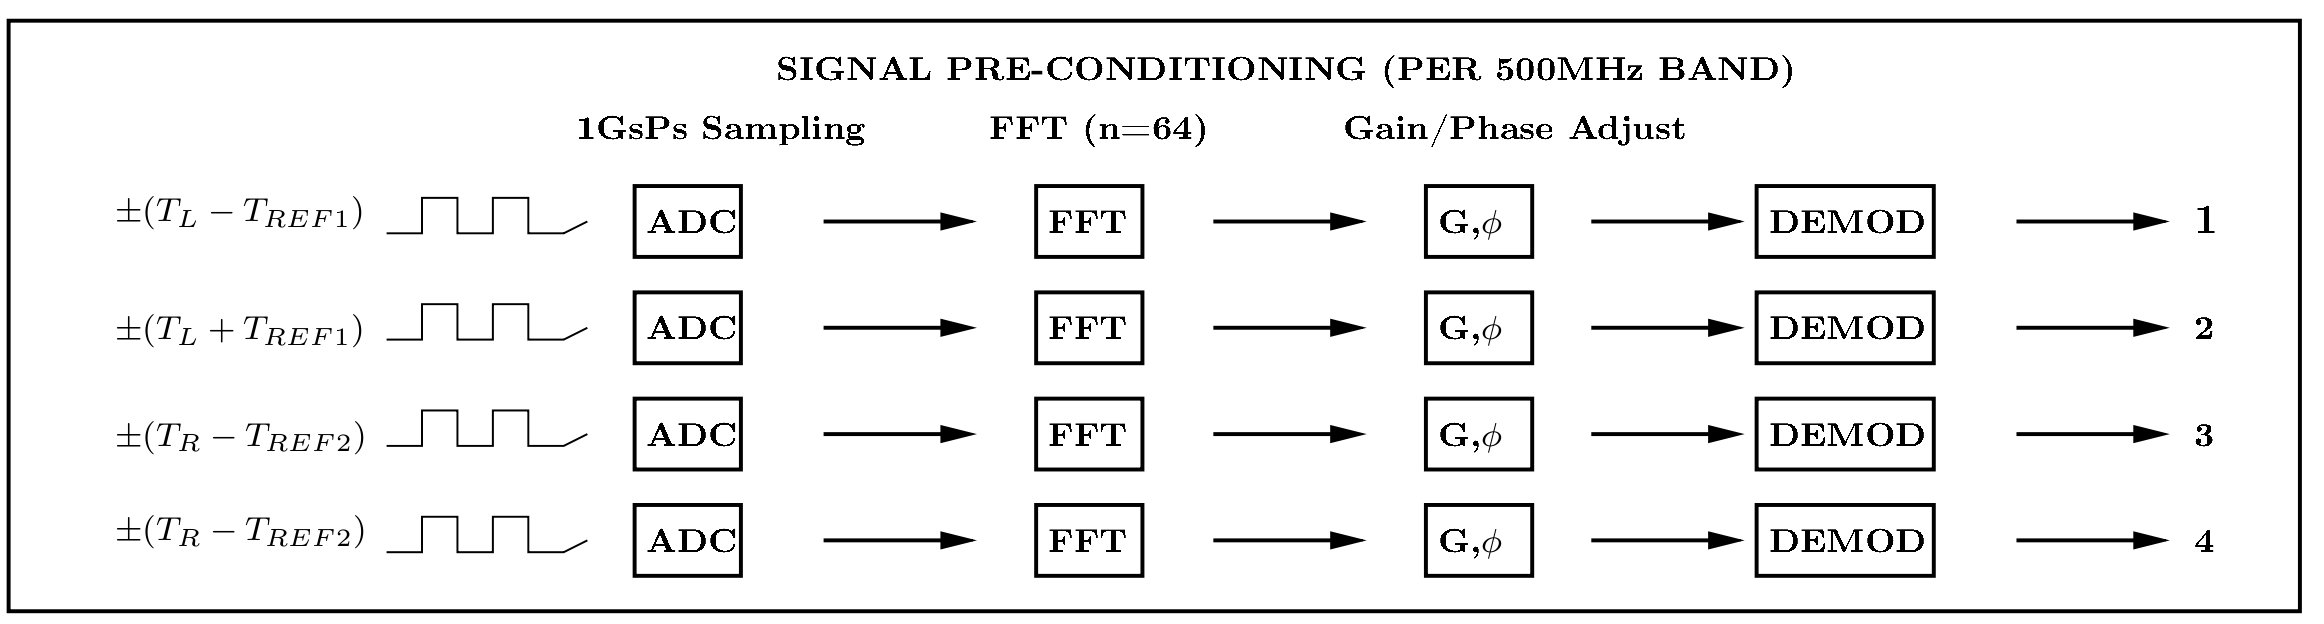
\includegraphics[width=\textwidth]{images/receiver_schematics/precon.jpg}\\
 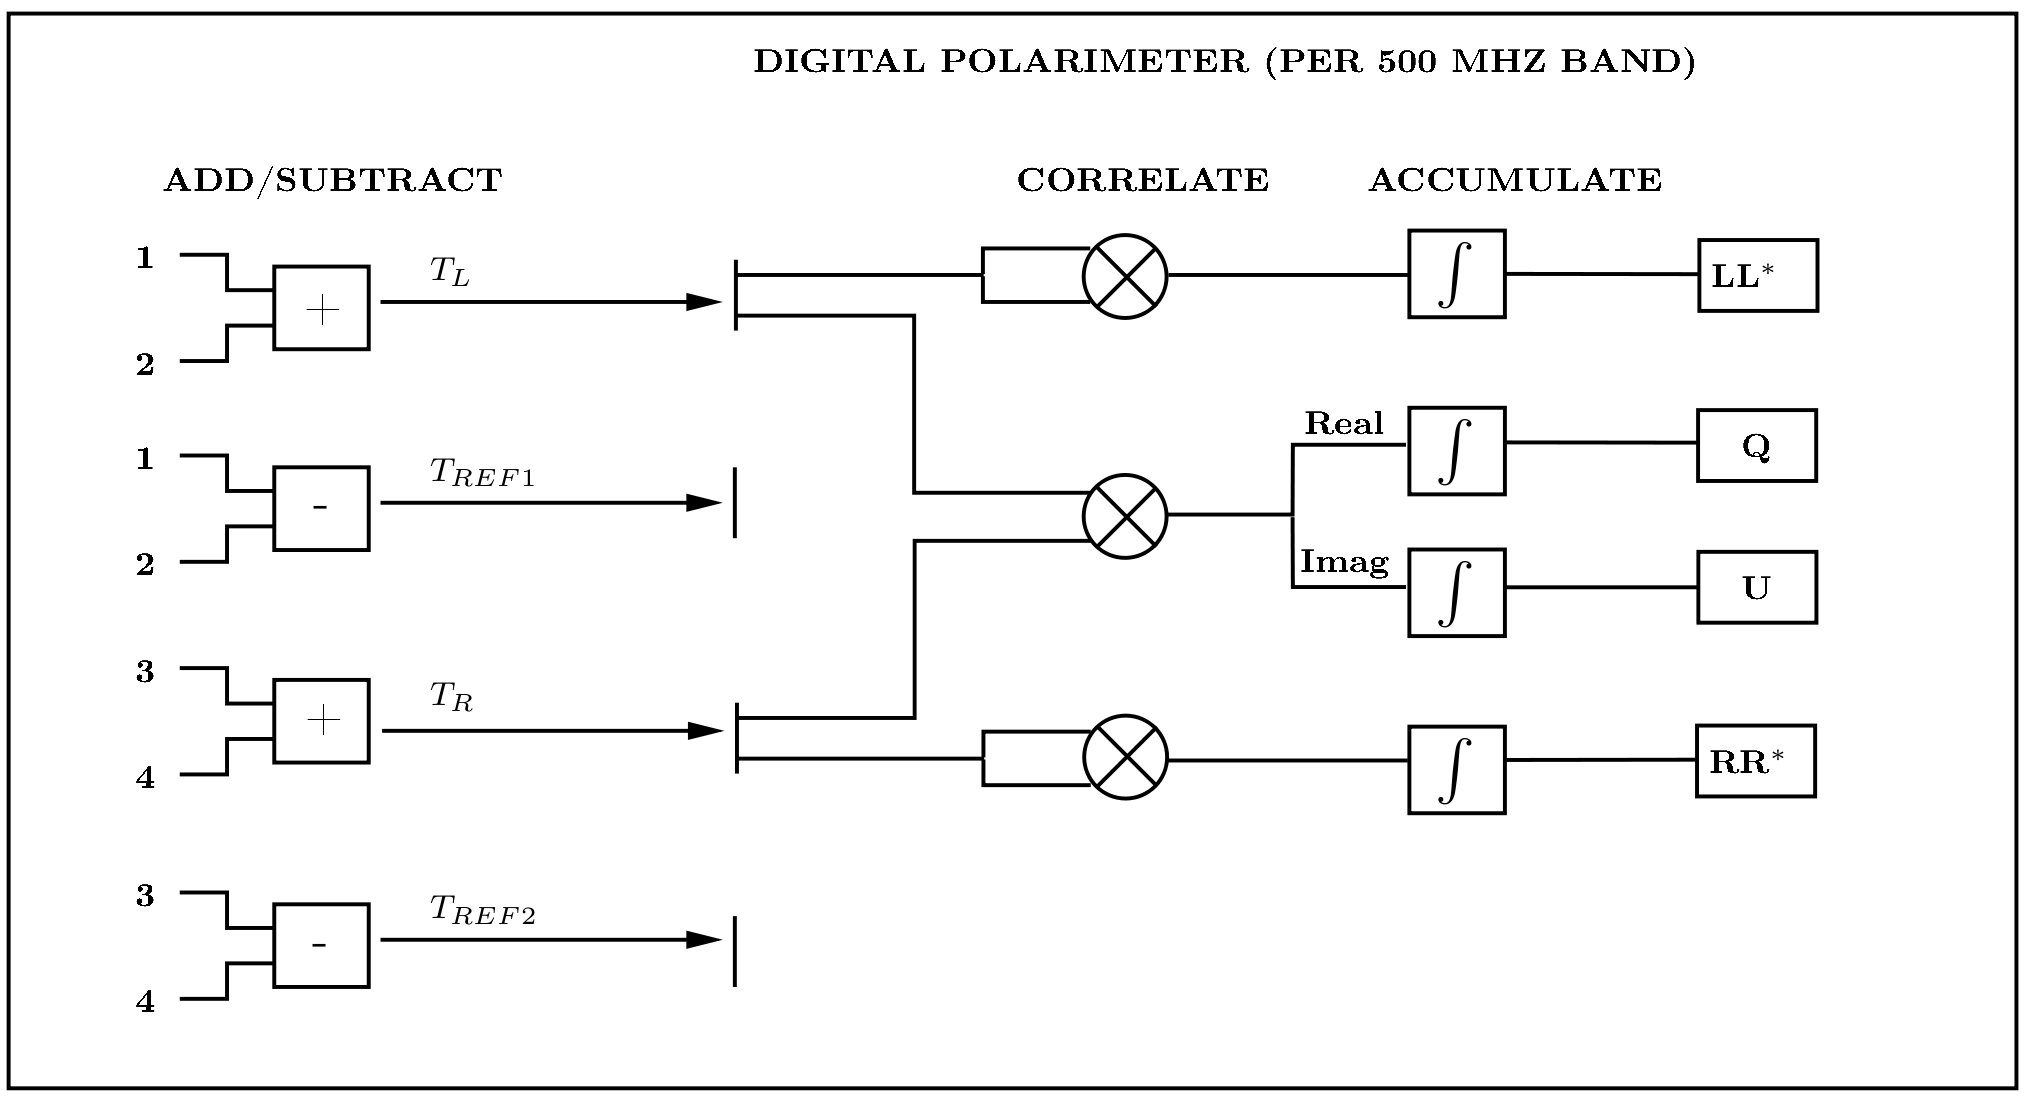
\includegraphics[width=\textwidth]{images/receiver_schematics/roach.jpg}
 % analog.png: 1920x1200 pixel, 72dpi, 67.73x42.33 cm, bb=
 \caption{Diagram of the digital polarimeter. The diagram shows one of the 500~MHz bands. The signals are sampled, fast-Fourier transformed, gain and phase adjusted, demodulated, added, correlated and then accumulated to produce the values required for the Stokes parameters. See \appen{sec:stokes}, Equations~\ref{eq:stokes_circ_I}$\rightarrow$\ref{eq:stokes_circ_V} for clarification on the correlations used to produce the Stokes parameters}
 \label{fig:digital_receiver_mine}
\end{figure}
\clearpage

Further information about the pseudo-correlation architecture employed is available in Appendix~\ref{sec:pseudoCorrelation}. This has been omitted from here for the purposes of this confirmation report. For reference a simplified block diagram of the digital receiver implementation is included in \fign{fig:digital_receiver} and \fign{fig:digital_receiver_mine}.


\subsection{Hardware State Summary}

The following list refers to \fign{fig:digital_receiver}.
\begin{itemize}
 \item Cryostat: Built, tested cool. Still needs temperature controller (Manchester)
 \item Orthomode Transducer (OMT): Built and ready for integration (Oxford)
 \item Linear to circular (L2C): Built and ready for integration (Oxford)
 \item 30dB  Couplers: Purchase and ready for integration (Oxford)
 \item $180^{\circ}$ hybrids: built and ready for integration (Oxford)
 \item Low noise amplifiers (LNA): still to be completed (Manchester)
 \item Warm amplifiers: built and integrated into backend 19 inch rack/power supply (Oxford)
 \item Phase Switches: built, not yet integrated into backend (Oxford).
 \item Band pass filters: built and integrated into backend (Oxford)
 \item Noise Diode: Purchased and integrated into backend (Oxford)
 \item Down Mixers: Built and integrated into backend (Oxford) (see \appen{sec:mixers})
 \item Two way splitters: Have components- might change design slightly and move splitter before the mixer. This will result in better isolation between the $0\rightarrow500$~MHz and $500\rightarrow1000$~MHz channels. (Oxford)
 \item Filters: 0-500MHz done. Currently finalising 500-1000MHz filter (Oxford) (see \appen{sec:lowfreqFilters})

\end{itemize}








% \section{Short Term Project Time-line}
% We are beginning to capture data at the OVRO site in California with the intention of mapping in the very near future. The design of the digital receiver is currently under way and we are optimistic about an initial deployment and commissioning by August. A brief outline of the next year's anticipated milestones is included in Table~\ref{tab:timeline}.
% 
% \begin{table}[ht]
% \caption{Revised C-BASS deployment time-line for 2010}
% 
% \begin{tabular}{l l l l }
% \\
% Year & Start Month & End Month & Description \\
% \hline\\
% 2010 & March & April & Preliminary digital design\\
% 2010 & April & Ongoing & Maps using the OVRO antenna \\
% 2010 & May & August & Assemble new receiver at Oxford \\
% 2010 & August & September & Deploy new receiver at OVRO, OVRO receiver to HartRAO \\
% 2010 & September & October & Commissioning  \\
% 2010 & October & Ongoing & Map making begins using both antennas
% \end{tabular} 
% 
% \label{tab:timeline}
% \end{table}





\clearpage


\clearpage
\subsection{Software and FPGA Firmware Status}

The integration of the backend control and data acquisition into the OVRO control system is the next logical step. We have thought carefully about how this will be undertaken, and believe the process will be straighforward, following a similar approach to our previous integration of the servo control last year.

The FPGA firmware design and implementation is nearly complete. All that remains is to implement the phase switching scheme. Demonstration results are included in \secn{sec:roachTests}.

\begin{figure}
\centering
\subfloat[The top half of the analog part of the digital receiver including the 4.5$\rightarrow$5.0~GHz bandpass filter, 4.5~GHz local oscillator, down mixers, splitter, 0$\rightarrow$500~MHz low pass filter, 500$\rightarrow$1000~MHz band pass filters. This tray will be temperature controlled]{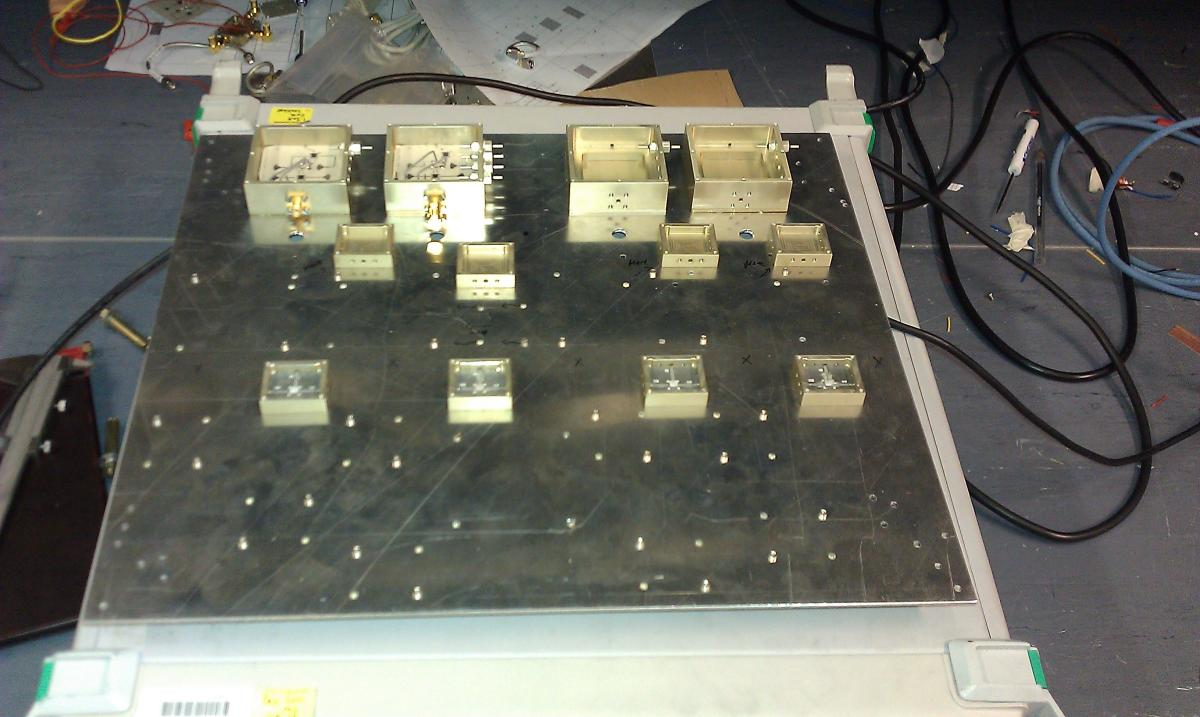
\includegraphics[width=0.5\textwidth]
{./images/digitalReceiver/IMAG0317a.jpg}
\label{fig:analogTrayForDigitala}
}
\subfloat[The bottom half of the same tray]{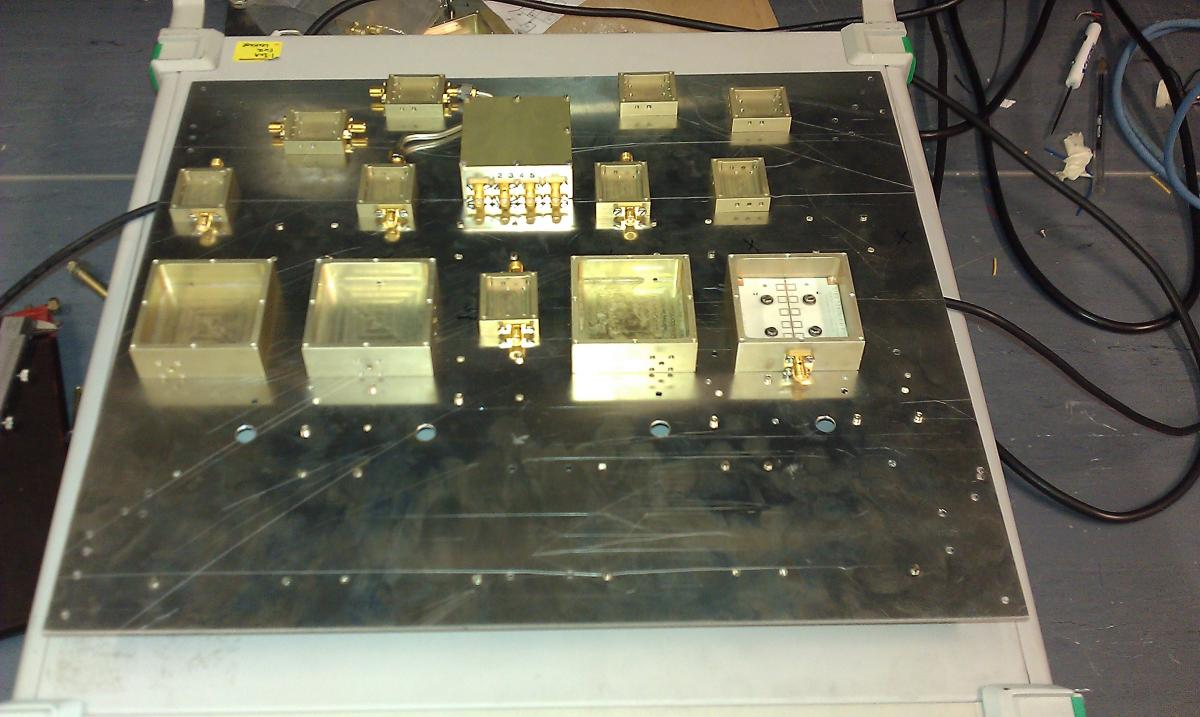
\includegraphics[width=0.5\textwidth]
{./images/digitalReceiver/IMAG0318a.jpg}
\label{fig:analogTrayForDigitalb}
}\\
 \subfloat[The digital receiver housing]{
 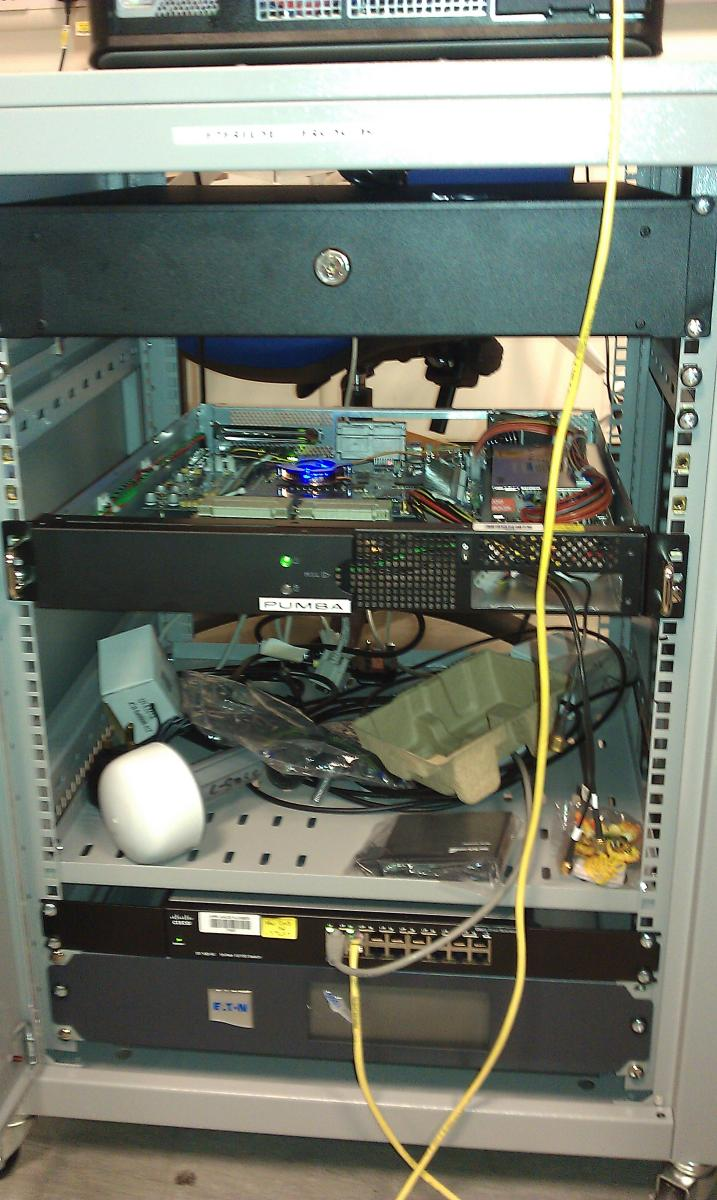
\includegraphics[height=0.5\textheight]{./images/digitalReceiver/IMAG0315a.jpg}
 \label{fig:rackForDigital}
}
\caption{Integration of the digital receiver. See \fign{fig:digital_receiver} for a diagram of the integrated system.}
\label{fig:digitalReceiverIntegration}


 % IMAG0315.jpg: 1952x3264 pixel, 72dpi, 68.86x115.15 cm, bb=0 0 1952 3264
 
\end{figure}

\clearpage
\subsection{Test Measurements}
\label{sec:roachTests}

Basic tests have been performed to check the performance of the FPGA backend. These have involved using a signal generator to inject a signal into the C-BASS RF chain, and using a phase delay chip to synthesise changing the phase between a nominal left and right circular polarisation. The test setup and results are described in \fign{fig:roachTest} and \fign{fig:rotating}, and have demonstrated the basic functionality of the backend.
\begin{figure}[ht]
 \centering
 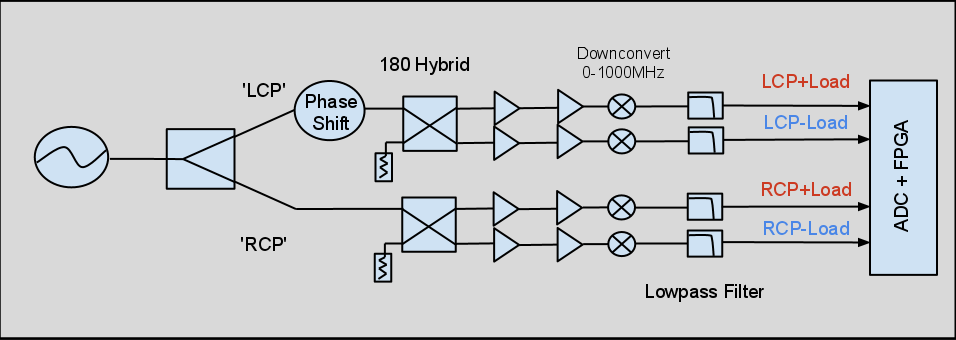
\includegraphics[width=\textwidth]{./images/RoachTests/TestSetupROACH.png}
 % TestSetupROACH.png: 956x340 pixel, 72dpi, 33.73x11.99 cm, bb=0 0 956 340
 \caption{Test Setup of RF test signal input to the ADC and ROACH board, producing a pseudo left (LCP) and right (RCP) circular polarisation signals, which are then injected into the RF chain already described in Section~\ref{sec:digitalRX}. If LCP and RCP are in phase we expect pure Q signal; if they are $90^{\circ}$ out of phase we expect pure U signal. See Appendix~\ref{sec:stokes},~Equation~\ref{eq:stokes_circ} for further details}
 \label{fig:roachTest}
\end{figure}



\begin{figure}[ht]
 \centering
\subfloat[][Intensity and Reference separation- see the separation between Intensity Channel 1/2 and Tref 1/2 in Channel Number 20]{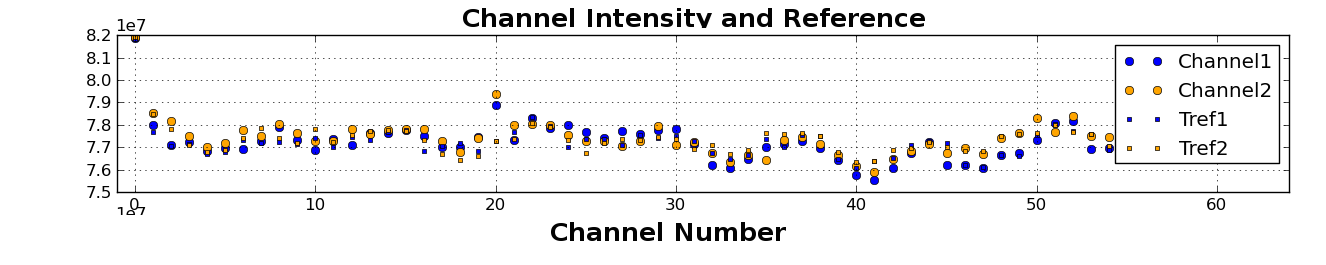
\includegraphics[width=\textwidth]{./images/RoachTests/Intensity.png}}\\
\subfloat[][Stokes Q and U with 0 degree rotation applied]{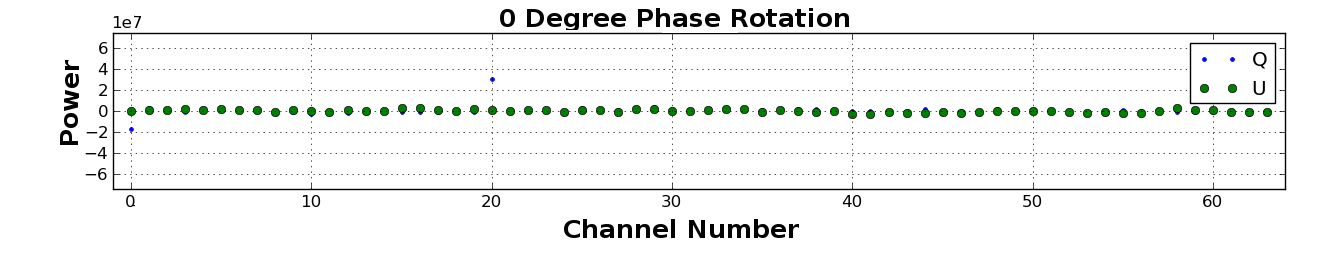
\includegraphics[width=\textwidth]{./images/RoachTests/17_1degreea.png}}\\
\subfloat[][$85^{\circ}$ rotation relative to (b)]{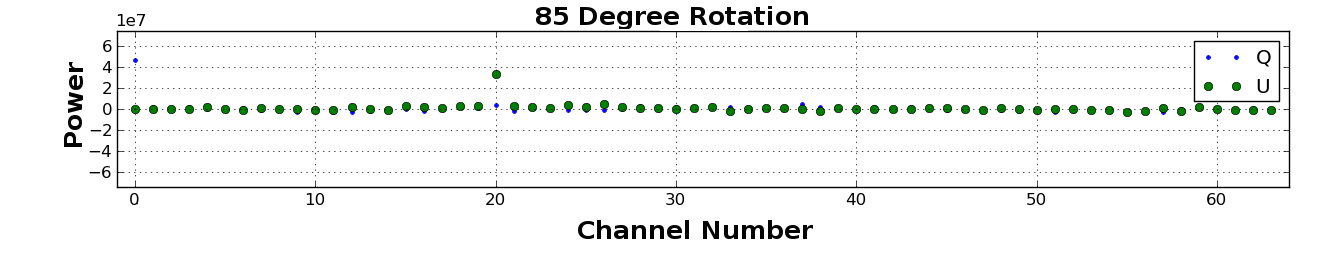
\includegraphics[width=\textwidth]{./images/RoachTests/102_6degreesa.png}}\\
\subfloat[][$102^{\circ}$ rotation relative to (b)]{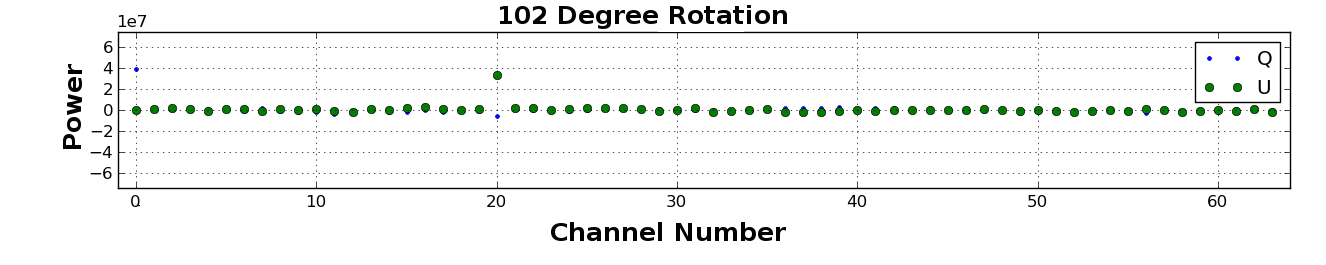
\includegraphics[width=\textwidth]{./images/RoachTests/119degreesa.png}}
 % 17_1degreea.png: 1326x265 pixel, 100dpi, 33.68x6.73 cm, bb=0 0 955 191
 \caption{Pure tone test signal used as input. This response is clearly evident in Channel 20. These plots show that the digital system successfully separates the Channel Intensity from Reference load (a), and that rotating the relative phases of the input signal through $90^{\circ}$ results in Stokes Q rotating into Stokes U as expected. Furthermore, we observe pure Stokes Q with no phase difference, and pure Stokes U with $90^{\circ}$ phase difference, as expected. For further information see Appendix~\ref{sec:stokes}}
 \label{fig:rotating}
\end{figure}

